\documentclass[sigconf]{acmart}
\settopmatter{printacmref=false}

%% remove copyright and further ACM refs for the Lab
\setcopyright{none}
\copyrightyear{}
\acmDOI{}
\acmISBN{}
\acmConference[Data Science Lab]{Data Science Lab}{2021}{Uni Passau}

%% end of the preamble, start of the body of the document source.
\begin{document}

%%
%% The "title" command has an optional parameter,
%% allowing the author to define a "short title" to be used in page headers.
\title{Trajectory prediction}

%% author list and team
\author{firstname lastname}
\email{mail@example.org}
\affiliation{\institution{}}
  
\author{firstname lastname}
\email{mail@example.org}
\affiliation{\institution{}}
  
\author{firstname lastname}
\email{mail@example.org}
\affiliation{\institution{}}
  
\author{Zubair Ahmed}
\email{ahmed08@ads.uni-passau.de}
\affiliation{\institution{}}

\renewcommand{\shortauthors}{Topic 3}

%%
%% The abstract is a short summary of the work to be presented in the
%% article.
\begin{abstract}
A generally good scheme for an abstract is the following:
\begin{itemize}
 \item The problem?
 \item Our solution.
 \item Our solution in detail.
 \item So what?
\end{itemize}
(1-2 sentences each). 
You don't need to provide an abstract during the first 3 phases, as you most likely will not have an answer to all items.
It should be included in your phase 4 submission and the final document.
\end{abstract}


%%
%% This command processes the author and affiliation and title
%% information and builds the first part of the formatted document.
\maketitle
\section*{Introduction}
This template should provide you some hints on preparing the reports. 
It is based on the template as provided by ACM\footnote{\url{https://www.acm.org/publications/proceedings-template}}.

When you submit the report, indicate who is responsible for a particular phase (either add the name to the section heading of the phase or add a section indicating all the phase responsibles).

Remove the irrelevant sections before submission.
Your submission for phase 1 should only contain the first section (Problem Statement) and References (and potentially the abstract).
Extend the document for the further phases, i.e. the submission for phase 2 should contain section 1 (Problem Statement) and 2 (Data Acquisition) and so on.

Submit the pdf version of your report to all tutors via e-mail:
\begin{itemize}
 \item sahib.julka@uni-passau.de
 \item julian.stier@uni-passau.de
 \item joerg.schloetterer@uni-passau.de
\end{itemize}


\section{Problem statement}
Describe your problem statement clearly and short.
Your algorithm will most likely not bring world-peace, but solve a particular problem.
Narrow down your problem to be as specific as possible. 
The more specific your problem, the better the chance to find a suitable solution. After a solution is found, the complexity can still be increased.
For example ``the beer price is too high, we aim to reduce it'' is not a very precise problem statement. What is ``too high''? Which kind of beer? At which area/country? At which occasion (restaurant,supermarket,special event,etc.)? ...?

Besides the problem statement, you should also indicate your approach on how you plan to solve it and how you plan to evaluate your solution in this section.

Most likely, the problem you are going to address is not completely new, but at least a similar problem has previously been addressed by others already.
Therefore, research how others solved this or similar problems, i.e. get familiar with the state of the art and related work.
You may then apply (and adapt/extend) an existing solution to a similar problem to your problem at hand.

\section{Data Acquisition \& Pre-Processing}
Make sure to precisely describe what you did and why.
The reader of your report should be able to reproduce the steps.
Therefore, it is for example not sufficient if you write ``we tokenized the sentences''.
You need to describe how the tokenization was done exactly, i.e. which regular expression or library/method you used with which parameters.

Frameworks/libraries are mentioned in footnotes instead of in the references section.
For example ``we used the \emph{TweetTokenizer} from the NLTK\footnote{\url{https://www.nltk.org/api/nltk.tokenize.html}} toolkit with the default parameters to tokenize our tweets''.

Reasoning is highly important. 
It should be obvious to the reader, why you do something in a particular way.
The following subsections provide hints on what to include in your report.

\begin{center}
 \noindent\fbox{%
    \parbox{0.3\textwidth}{%
        (!) required \newline
        (*) if it applies to your project
    }%
}

\end{center}

\subsection{Data acquisition}
\begin{itemize}
 \item source of data (!)
 \item means of acquisition (!)
 \item reasoning (!) (i.e. why you chose that kind of data, that source, why you crawled it in that way, etc.)
\end{itemize}
As the datasets are mostly pre-defined (i.e. in most of the topics you do not need to acquire the data yourself), this part can be short.

\subsection{Data preprocessing}
\begin{itemize}
 \item filtering / grouping / labeling (*)
 \item lemmatization/stemming (*)
 \item other (*)
 \item statistics on the data (!) (e.g. volume, classes, distributions, correlations, etc.)
 \item reasoning (!)
\end{itemize}

\subsection{Feature engineering}
\begin{itemize}
 \item input x and output y of the system (*)
 \item feature extraction (*)
 \item feature transformation (*)
 \item reasoning (!)
\end{itemize}



\section{Model implemenation}
\subsection{Methodology / Proposed solution / Technique}
An in-depth description of your solution to the problem. (e.g. input - output, system description, ML techniques, etc.)

\subsection{Experimental Setup}
An in-depth description of the experimental design which enables an objective quantification of the quality of your solution. (e.g. dataset, baselines, metrics, etc.).
Might be moved to the next section (Phase 4).

\section{Evaluation}
\subsection{Results}
The evaluation of your solution by means of the experiments. 
Figures and statistics provide hard facts about the quality of your solution from different viewpoints.

\subsection{Discussion}
So what? 
How well could we solve the problem? 
What are the limitations? 
Open ends.


\section*{Template information (remove this section in your report)}
\label{sec:template-information}
Instructions in the following sections are included from the original ACM template sample file.
The article template's documentation, available at
\url{https://www.acm.org/publications/proceedings-template}, has a
complete explanation and tips for effective use.

\subsection*{Sectioning Commands}

Your work should use standard \LaTeX\ sectioning commands:
\verb|section|, \verb|subsection|, \verb|subsubsection|, and
\verb|paragraph|. 

\subsection*{Tables}

The ``\verb|acmart|'' document class includes the ``\verb|booktabs|''
package --- \url{https://ctan.org/pkg/booktabs} --- for preparing
high-quality tables.

Table captions are placed {\itshape above} the table.

Because tables cannot be split across pages, the best placement for
them is typically the top of the page nearest their initial cite.  To
ensure this proper ``floating'' placement of tables, use the
environment \textbf{table} to enclose the table's contents and the
table caption.  The contents of the table itself must go in the
\textbf{tabular} environment, to be aligned properly in rows and
columns, with the desired horizontal and vertical rules.  Again,
detailed instructions on \textbf{tabular} material are found in the
\textit{\LaTeX\ User's Guide}.

Immediately following this sentence is the point at which
Table~\ref{tab:freq} is included in the input file; compare the
placement of the table here with the table in the printed output of
this document.

\begin{table}
  \caption{Frequency of Special Characters}
  \label{tab:freq}
  \begin{tabular}{ccl}
    \toprule
    Non-English or Math&Frequency&Comments\\
    \midrule
    \O & 1 in 1,000& For Swedish names\\
    $\pi$ & 1 in 5& Common in math\\
    \$ & 4 in 5 & Used in business\\
    $\Psi^2_1$ & 1 in 40,000& Unexplained usage\\
  \bottomrule
\end{tabular}
\end{table}

To set a wider table, which takes up the whole width of the page's
live area, use the environment \textbf{table*} to enclose the table's
contents and the table caption.  As with a single-column table, this
wide table will ``float'' to a location deemed more
desirable. Immediately following this sentence is the point at which
Table~\ref{tab:commands} is included in the input file; again, it is
instructive to compare the placement of the table here with the table
in the printed output of this document.

\begin{table*}
  \caption{Some Typical Commands}
  \label{tab:commands}
  \begin{tabular}{ccl}
    \toprule
    Command &A Number & Comments\\
    \midrule
    \texttt{{\char'134}author} & 100& Author \\
    \texttt{{\char'134}table}& 300 & For tables\\
    \texttt{{\char'134}table*}& 400& For wider tables\\
    \bottomrule
  \end{tabular}
\end{table*}

\subsection*{Math Equations}
You may want to display math equations in three distinct styles:
inline, numbered or non-numbered display.  Each of the three are
discussed in the next sections.

\subsubsection*{Inline (In-text) Equations}
A formula that appears in the running text is called an inline or
in-text formula.  It is produced by the \textbf{math} environment,
which can be invoked with the usual
\texttt{{\char'134}begin\,\ldots{\char'134}end} construction or with
the short form \texttt{\$\,\ldots\$}. You can use any of the symbols
and structures, from $\alpha$ to $\omega$, available in
\LaTeX~\cite{Lamport:LaTeX}; this section will simply show a few
examples of in-text equations in context. Notice how this equation:
\begin{math}
  \lim_{n\rightarrow \infty}x=0
\end{math},
set here in in-line math style, looks slightly different when
set in display style.  (See next section).

\subsubsection*{Display Equations}
A numbered display equation---one set off by vertical space from the
text and centered horizontally---is produced by the \textbf{equation}
environment. An unnumbered display equation is produced by the
\textbf{displaymath} environment.

Again, in either environment, you can use any of the symbols and
structures available in \LaTeX\@; this section will just give a couple
of examples of display equations in context.  First, consider the
equation, shown as an inline equation above:
\begin{equation}
  \lim_{n\rightarrow \infty}x=0
\end{equation}
Notice how it is formatted somewhat differently in
the \textbf{displaymath}
environment.  Now, we'll enter an unnumbered equation:
\begin{displaymath}
  \sum_{i=0}^{\infty} x + 1
\end{displaymath}
and follow it with another numbered equation:
\begin{equation}
  \sum_{i=0}^{\infty}x_i=\int_{0}^{\pi+2} f
\end{equation}
just to demonstrate \LaTeX's able handling of numbering.

\subsection*{Figures}

The ``\verb|figure|'' environment should be used for figures. One or
more images can be placed within a figure. If your figure contains
third-party material, you must clearly identify it as such, as shown
in the example below.
\begin{figure}[h]
  \centering
  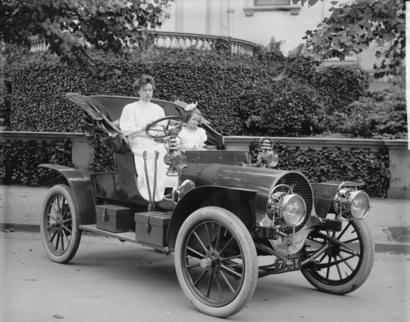
\includegraphics[width=\linewidth]{sample-franklin}
  \caption{1907 Franklin Model D roadster. Photograph by Harris \&
    Ewing, Inc. [Public domain], via Wikimedia
    Commons. (\url{https://goo.gl/VLCRBB}).}
  \Description{The 1907 Franklin Model D roadster.}
\end{figure}

Your figures should contain a caption which describes the figure to
the reader. 
Figure captions are placed {\itshape below} the figure.



\subsection*{Citations and Bibliographies}

The use of \emph{BibTeX} for the preparation and formatting of one's
references is strongly recommended. Authors' names should be complete
--- use full first names (``Donald E. Knuth'') not initials
(``D. E. Knuth'') --- and the salient identifying features of a
reference should be included: title, year, volume, number, pages,
article DOI, etc.

The bibliography is included in your source document with these two
commands, placed just before the \verb|\end{document}| command:
\begin{verbatim}
  \bibliographystyle{ACM-Reference-Format}
  \bibliography{bibfile}
\end{verbatim}
where ``\verb|bibfile|'' is the name, without the ``\verb|.bib|''
suffix, of the \emph{BibTeX} file.

  Some examples.  A paginated journal article \cite{Abril07}, an
  enumerated journal article \cite{Cohen07}, a reference to an entire
  issue \cite{JCohen96}, a monograph (whole book) \cite{Kosiur01}, a
  monograph/whole book in a series (see 2a in spec. document)
  \cite{Harel79}, a divisible-book such as an anthology or compilation
  \cite{Editor00} followed by the same example, however we only output
  the series if the volume number is given \cite{Editor00a} (so
  Editor00a's series should NOT be present since it has no vol. no.),
  a chapter in a divisible book \cite{Spector90}, a chapter in a
  divisible book in a series \cite{Douglass98}, a multi-volume work as
  book \cite{Knuth97}, an article in a proceedings (of a conference,
  symposium, workshop for example) (paginated proceedings article)
  \cite{Andler79}, a proceedings article with all possible elements
  \cite{Smith10}, an example of an enumerated proceedings article
  \cite{VanGundy07}, an informally published work \cite{Harel78}, a
  doctoral dissertation \cite{Clarkson85}, a master's thesis:
  \cite{anisi03}, an online document / world wide web resource
  \cite{Thornburg01, Ablamowicz07, Poker06}, a video game (Case 1)
  \cite{Obama08} and (Case 2) \cite{Novak03} and \cite{Lee05} and
  (Case 3) a patent \cite{JoeScientist001}, work accepted for
  publication \cite{rous08}, 'YYYYb'-test for prolific author
  \cite{SaeediMEJ10} and \cite{SaeediJETC10}. Other cites might
  contain 'duplicate' DOI and URLs (some SIAM articles)
  \cite{Kirschmer:2010:AEI:1958016.1958018}. Boris / Barbara Beeton:
  multi-volume works as books \cite{MR781536} and \cite{MR781537}. A
  couple of citations with DOIs:
  \cite{2004:ITE:1009386.1010128,Kirschmer:2010:AEI:1958016.1958018}. Online
  citations: \cite{TUGInstmem, Thornburg01, CTANacmart}.


\subsection*{Appendices}

If your work needs an appendix, add it before the
``\verb|\end{document}|'' command at the conclusion of your source
document.

Start the appendix with the ``\verb|appendix|'' command:
\begin{verbatim}
  \appendix
\end{verbatim}
and note that in the appendix, sections are lettered, not
numbered. This document has two appendices, demonstrating the section
and subsection identification method.


%%
%% The next two lines define the bibliography style to be used, and
%% the bibliography file.
\bibliographystyle{ACM-Reference-Format}
\bibliography{references}

%%
%% If your work has an appendix, this is the place to put it.
\appendix

\section{Research Methods (remove if not used)}

\subsection{Part One}

Lorem ipsum dolor sit amet, consectetur adipiscing elit. Morbi
malesuada, quam in pulvinar varius, metus nunc fermentum urna, id
sollicitudin purus odio sit amet enim. Aliquam ullamcorper eu ipsum
vel mollis. Curabitur quis dictum nisl. Phasellus vel semper risus, et
lacinia dolor. Integer ultricies commodo sem nec semper.

\subsection{Part Two}

Etiam commodo feugiat nisl pulvinar pellentesque. Etiam auctor sodales
ligula, non varius nibh pulvinar semper. Suspendisse nec lectus non
ipsum convallis congue hendrerit vitae sapien. Donec at laoreet
eros. Vivamus non purus placerat, scelerisque diam eu, cursus
ante. Etiam aliquam tortor auctor efficitur mattis.

\section{Online Resources}

Nam id fermentum dui. Suspendisse sagittis tortor a nulla mollis, in
pulvinar ex pretium. Sed interdum orci quis metus euismod, et sagittis
enim maximus. Vestibulum gravida massa ut felis suscipit
congue. Quisque mattis elit a risus ultrices commodo venenatis eget
dui. Etiam sagittis eleifend elementum.

Nam interdum magna at lectus dignissim, ac dignissim lorem
rhoncus. Maecenas eu arcu ac neque placerat aliquam. Nunc pulvinar
massa et mattis lacinia.

\end{document}
